\documentclass[11pt,letter]{article}
\usepackage{amsmath}
\usepackage{amssymb}	% packages that allow mathematical formatting
\usepackage{graphicx}	% package that allows you to include graphics
\usepackage{setspace}	% package that allows you to change spacing
\usepackage{fullpage}	% package that specifies normal margins
\usepackage{microtype}
\usepackage{amsthm}
\newcommand{\argmin}{\operatornamewithlimits{argmin}}
\renewcommand\qedsymbol{$\blacksquare$}
\usepackage{listings}
\usepackage{color}
\usepackage{subfig}


\definecolor{codegreen}{rgb}{0,0.6,0}
\definecolor{codegray}{rgb}{0.5,0.5,0.5}
\definecolor{codepurple}{rgb}{0.58,0,0.82}
\definecolor{backcolour}{rgb}{0.95,0.95,0.95}

\lstdefinestyle{mystyle}{
	backgroundcolor=\color{backcolour},   
	commentstyle=\color{codegreen},
	keywordstyle=\color{magenta},
	numberstyle=\tiny\color{codegray},
	stringstyle=\color{codepurple},
	basicstyle=\footnotesize,
	breakatwhitespace=false,         
	breaklines=true,                 
	captionpos=b,                    
	keepspaces=true,                 
	numbers=left,                    
	numbersep=5pt,                  
	showspaces=false,                
	showstringspaces=false,
	showtabs=false,                  
	tabsize=2
}

\lstset{style=mystyle}

%\usepackage[left=2.5cm, right=2.5cm, top=2cm, bottom = 3cm]{geometry}


	

\begin{document}
\title{FNCE 924 Problem Set 1}
\author{Patrick Shultz }
\date{\today}
\maketitle 
\noindent\large\textbf{Part I: Consumption Choices}
\section*{Problem 1}
\paragraph{a)}
Consumer maximizes
\begin{equation*}
	U = E_0\left[ \sum_{t = 0}^{\infty} \beta^t( u(a+ \theta_t)c_t - bc_t^2)\right] 
\end{equation*}
subject to $c_t = Rk_t + y_t - k_{t+1}$ and where $R = 1/\beta$ and the shock $\theta$ captures taste shocks to the marginal utility of consumption. Denoting the value of future periods with ``$'$", the objective function and budget constraint imply the Lagrangian is
\begin{equation*}
	\mathcal{L} = u(c) +\beta E\left[V(k', y', R') \right] + \lambda \left[Rk + y - c-k' \right]  
\end{equation*}
First order conditions for $c$ and $k'$:
\begin{equation*}
	\begin{split}
	 u_c(c) - \lambda &=0\\
	\beta E_{y, R}\left[ V_k(k', y', R')\right]-\lambda &= 0\\
	\end{split}
\end{equation*}
Differentiating the value function with respect to $k$ gives the Envelope condition
\begin{equation*}
\begin{split}
V_k(k, y, R) &= R\lambda\\  
\end{split}
\end{equation*}
The FOCs with respect to $c$ and the Envelope condition with respect to $k$ imply the Euler equation 
\begin{equation*}
	u_c(c) = \beta E_{y, R} V_k(k', y', R)
\end{equation*}
Iterating forward one time period on the Envelope condition gives
\begin{equation*}
\begin{split}
u_c(c) &= \beta E_{y, R} R u_c(c')\\
&= E_{y} u_c(c')\\
\end{split}
\end{equation*}
where $u_c(c) = (a+\theta) + 2bc$, so our Euler equation is 
\begin{equation}
a + \theta_t - 2bc_t = E_t\left[a + \theta_{t+1} -2bc_{t+1} \right]  
\end{equation}

\paragraph{b)} Assuming $\theta_{t}$ follows an AR(1) process with mean 0, we can characterize the process for optimal consumption as follows. Let $\theta_t = \phi \theta_{t-1} + \epsilon_t$ where$|\phi| <1$, so the series converges.  Solving for $c_t$, we can then  rewrite the Euler equation as 
\begin{equation}
\begin{split}
	c_t & = E_t c_{t+1}+\bigg(\frac{(1-\phi)\theta_t}{2b}\bigg)\\
	&=E_t\left[  c_{t+2} + \bigg(\frac{(1-\phi)\theta_{t+1}}{2b}\bigg)\right] +\bigg(\frac{(1-\phi)\theta_t}{2b}\bigg)\\
	&= E_t\left[  c_{t+s}\right] +\bigg(\frac{(1-\phi)}{2b}\bigg)\sum_{s = 1}^{\infty}\phi^{s-1}\theta_t\\
	&= E_t\left[  c_{t+s}\right] +\bigg(\frac{(1-\phi)}{2b}\bigg)\frac{\theta_t}{1-\phi}\\
	&= E_t\left[c_{t+s}\right] + \frac{\theta_t}{2b}\\
\end{split}
\label{eq:opt_c_AR1}
\end{equation}
By iterating back to the initial condition,  equation (\ref{eq:opt_c_AR1})  implies $E_0\left[c_{t}\right] = c_0 -\frac{\theta_0}{2b}$. 
We now consider the lifetime budget constraint to characterize the process for optimal consumption. 	
\begin{equation*}
\begin{split}
Rk_0 + \sum_{j = 0}^{\infty}R^{-t}E_0\left[ y_t\right] &= \sum_{t=0}^{\infty}R^{-t}E_0\left[c_t\right]\\
\implies Rk_0 + \sum_{t=0}^{\infty}R^{-t}E_0\left[y_t\right]  &= \frac{R}{R-1}\bigg(c_0 -\frac{\theta_0}{2b}\bigg)\\
\implies \frac{R-1}{R}\bigg(Rk_0 + \sum_{t = 0}^{\infty}R^{-t}E_0\left[y_t\right]\bigg) +\frac{\theta_0}{2b} &= c_0\\
\end{split}
\end{equation*}
where the second line holds from the Euler equation. If we assume the process of $y$ satisfies the Markov property, we have characterized consumption as a function of current state variables. This is the same solution as the deterministic case, but with an additional factor to take into account initial tastes and one of the parameters of the quadratic utility function. 
\paragraph{c)} We now assume our process for $\theta$ is given by $\theta_{t+1} = \theta_t + \epsilon_{t+1}$, a random walk. Solving for $c_t$, we can rewrite the Euler equation as
\begin{equation*}
\begin{split}
	a + \theta_t - 2bc_t &= E_t\left[a + \theta_{t+1} - 2bc_{t+1}\right]\\
	&=  E_t\left[a + \theta_{t}+ \epsilon_{t+1} - 2bc_{t+1}\right]\\
	\implies c_t &=E_t\left[c_{t+1}\right]
\end{split}
\end{equation*}
Thus, when taste shocks follow a random walk,  we are back in the case where consumption is a random walk.The lifetime budget constaint is
\begin{equation*}
	\begin{split}
	Rk_0 + \sum_{t = 0}^{\infty}R^{-t}E_0\left[y_t\right] = \sum_{t = 0}^{\infty}R^{-t}E_0\left[c_t\right]\\
	Rk_0 + \sum_{t = 0}^{\infty}R^{-t}E_0\left[y_t\right] = \frac{R}{R-1}c_0\\
	c_0 = \frac{R-1}{R}\bigg(Rk_0 + \sum_{t = 0}^{\infty}R^{-t}E_0\left[y_t\right]\bigg)
	\end{split}
\end{equation*}
Once again, we assume $y$ satisfies the Markov property.
\paragraph{d)} Assume $\beta R < 1$  and $\theta$ is a random walk. The Euler equation gives
\begin{equation*}
\begin{split}
	a + \theta_t + 2bc_t = \beta R E_t\left[a + \theta_{t+1} + 2b c_{t+1}\right]\\
	\implies -2bc_t = a(\beta R -1) + \theta_t(\beta R -1) - 2bE_t\left[c_{t+1}\right]\\
	\implies c_t = \bigg(\frac{1-\beta R}{2b}\bigg)(a + \theta_{t}) + E_t\left[c_{t+1}\right]
	\end{split}
\end{equation*}
Iterating forward on $ c_t = \bigg(\frac{1-\beta R}{2b}\bigg)(a+\theta_t) + E_t\left[c_{t+1}\right]$ yields 
\begin{equation*}
	c_t = E_t\left[c_{t+s}\right] + s\bigg(\frac{1-\beta R}{2b}\bigg)(a + \theta_{t})
\end{equation*}
Intuitively, this implies that when $\beta R < 1$ the rate of return on savings is too low, so an agent will consume relatively more than in comparison to the case when $\beta R =1$. Plugging into the lifetime budget constraint, we get
\begin{equation*}
\begin{split}
	Rk_0 + \sum_{t = 0}^{\infty}R^{-t}E_0\left[y_t\right] &= \sum_{t = 0}^{\infty}R^{-t}E_0\left[c_t\right]\\
	Rk_0  + \sum_{t = 0}^{\infty}R^{-t}E_0\left[y_t\right] &= \sum_{t = 0}^{\infty}R^{-t}\bigg(c_0 - t \bigg(\frac{1-\beta R}{2b}\bigg)(a + \theta_0)\bigg)\\
	Rk_0  + \sum_{t = 0}^{\infty}R^{-t}E_0\left[y_t\right] &= \frac{R}{R-1}c_0 - \sum_{t = 0}^{\infty}R^{-t}\bigg(t \bigg(\frac{1-\beta R}{2b}\bigg)(a + \theta_0)\bigg)\\
\end{split}
\end{equation*}
We can solve this expression for consumption and  see that our optimal consumption process is given by the following
\begin{equation}
\begin{split}
	c_0 &= \frac{R-1}{R} \bigg[Rk_0  + \sum_{t = 0}^{\infty}R^{-t}E_0\left[y_t\right] + \sum_{t = 0}^{\infty}R^{-t}\bigg(t \bigg(\frac{1-\beta R}{2b}\bigg)(a + \theta_0)\bigg)\bigg]\\&= \frac{R-1}{R} \bigg[Rk_0  + \sum_{t = 0}^{\infty}R^{-t}E_0\left[y_t\right] + \frac{R}{(R-1)^2}\bigg( \bigg(\frac{1-\beta R}{2b}\bigg)(a + \theta_0)\bigg)\bigg]
\end{split}
\end{equation}
\section*{Problem 2}
We now consider the optimization problem of an individual that can invest in human capital to get a return rate, $A_t$, in units of the consumption good. The agent's problem is
\begin{equation*}
	V = E_0\left[\sum_{t=0}^{\infty}\beta^t \log(c_t)\right]
\end{equation*}
subject to the budget constraint $c_t + h_{t+1} = A_t h_t$. 
\paragraph{a)}
We use a Bellman equation to specify the recursive formulation of this problem:
\begin{equation*} \label{Problem2}
V(h_t, A_t) = \underset{c_t,h_{t+1}}{\max}\{\log(c_t) + \beta E_t\left[ V((h_{t+1}, A_{t+1}))\right] \} \text{ s.t. } c_t = A_th_t-h_{t+1}
\end{equation*}
Since we are given that $A_t$ follows a first order Markov process, we see that this is recursive problem. 
\paragraph{b)}
We first conjecture the solution to our problem can be written as 
\begin{equation*}
	V(h_t, A_t) = E_t\left[\sum_{t=s}^{\infty}\beta^{s-t} \log(c_t^*)\right]
\end{equation*}
where $c_t^*$ denotes optimal consumption and show that this expression is satisfied by $V(h, A) = \alpha\log(h) + v(A)$  by showing it is a fixed point for our problem. 
\begin{align*}
V(h_t, A_t)	&= \underset{c_t,h_{t+1}}{\max}\{\log(c_t) + \beta E_t\left[V(h_{t+1}, A_{t+1})\right] \}\\
&= \underset{c_t,h_{t+1}}{\max}\{\log(c_t) + \beta E_t\left[ \alpha \log(h_{t+1}) + v(A_{t+1}))\right] \}\\
&= \underset{c_t,h_{t+1}}{\max}\{\log(c_t) - \log(h_t) + \log(h_t) + \beta E_t\left[ \alpha (\log(h_{t+1}) - \log(h_t) + \log(h_t)) + v(A_{t+1}))\right] \}\\
&= (1+\beta a)\log(h_t) + \underset{\hat{c}_t,\hat{h}_{t+1}}{\max}\{\log(\hat{c}_t) + \beta E_t\left[ \alpha \log(\hat{h}_{t+1}) + v(A_{t+1}))\right] \} &(\star)\\
&= \underbrace{(1+\beta \alpha)}_{\equiv \alpha} \log(h_t) + \underbrace{ \beta E_t[v(A_{t+1})] + \max_{\hat{c}_t,\hat{h}_{t+1}}\{\log(\hat{c}_t) + \beta E_t\left[ \alpha \log(\hat{h}_{t+1})\right] \}}_{\equiv v(A_t)}\\
&= \alpha \log(h_t) + v(A_t)
\end{align*}
where $(\star)$ introduces the change of variables where variables are normalized by human capital investment: $\hat{c}_{t} = \frac{c_{t}}{h_{t}}$ and $\hat{h}_{t+1} = \frac{h_{t+1}}{h_{t}}$ and the constraint of the maximization problem is\\
\begin{equation*}
	\hat{c}_t + \hat{h}_{t+1} = A_t
\end{equation*}

Thus we have $\alpha = \frac{1}{1-\beta}$ and since the distribution of $A_{t+1}$ only depends on $A_t$, we can define $v(A_t)$ as the solution to the problem
\begin{equation*}
	v(A_t) = \beta E_t[v(A_{t+1})] + \max_{\hat{c}_t,\hat{h}_{t+1}}\{\log(\hat{c}_t) + \beta E_t\left[ \alpha \log(\hat{h}_{t+1})\right] \}
\end{equation*}

Thus, we have found a fixed point to our problem and have shown that the conjectured form holds. 


\paragraph{c)}
To find optimal consumption and human capital choices, we take the first order conditions with respect to $c_t$ and $h_t$ to get
\begin{equation}
0 = u_c(c_t) - \lambda
\label{eq:FOC}
\end{equation}
\begin{equation}\label{Env}
V_h(h_t, A_t) = \lambda A_t\\
\end{equation}
Equations (\ref{eq:FOC}), (\ref{Env}) and the value function imply
\begin{align*}
u_c(c_t)		&= V_h(h_t, A_t)\frac{1}{A_t}\\
&= \frac{\partial}{\partial h_t}(\alpha \log(h_t) + v(A_t))\frac{1}{A_t}\\
\frac{1}{c_t}	&= \alpha \frac{1}{h_t}\frac{1}{A_t}
\end{align*}
Since $\alpha = \frac{1}{1 - \beta}$, optimal consumption is a function of current state variables and known parameters
\begin{equation}
c_t^* = A_t h_t (1-\beta)
\end{equation}
Plugging $c_t^*$ into the budget constraint yields optimal human capital investment as a function of the current state variables and known parameters
\begin{equation}
h_{t+1}^*=A_t h_t \beta 
\label{eq:opt_human_capital_investment}
\end{equation}

\paragraph{d)}
Assuming $\log A \sim^{iid} N(\mu_A,\sigma^2)$ and using \ref{eq:opt_human_capital_investment}, we can solve for expected growth of human capital investments as follows
\begin{align*}
h_{t+1} 								&= \beta A_t h_t\\
\frac{h_{t+1}}{h_t} 					&= \beta A_t\\
\log\left[\frac{h_{t+1}}{h_t}\right] 	&= \log\beta +\log A_t\\
E_t \log\left[\frac{h_{t+1}}{h_t}\right] 	&= \log\beta + E_t \log A_t\\
E_t \log\left[\frac{h_{t+1}}{h_t}\right] 	&= \log\beta + \mu_A
\end{align*}
To solve for the consumption growth process, we use of the Euler equation,  $u_c(c_t) = \beta E_t [A_{t+1}u_c(c_{t+1})]$

\begin{align*}
\frac{1}{c_t} 	&= \beta E_t\left[ A_{t+1} \frac{1}{c_{t+1}} \right]\\
1				&= \beta E_t\left[ A_{t+1} \frac{c_t}{c_{t+1}} \right]\\
&= \beta E_t\left[ A_{t+1}\right] E_t\left[ \frac{c_t}{c_{t+1}} \right] \\
E_t\left[ \frac{c_{t+1}}{c_{t}} \right] &= \beta E_t\left[ A_{t+1} \right]\\
\log E_t\left[ \frac{c_{t+1}}{c_{t}} \right] &= \log \beta + \mu_A + \frac{1}{2}\sigma^2
\end{align*}
where we can split the expectation from lines two to three because $A$ is distributed iid. \\


\noindent\textbf{Part II: Numerical Methods}\\
We consider the following problem
\begin{equation*}
U = E_0\left[ \sum_{t = 0}^{\infty} \beta^t u(c_t)\right] 
\end{equation*}
subject to $c_t = Rk_t + y_t - k_{t+1}$ and $ k_0 > 0$. 
\section*{Problem 1} Assume that $\log(y)$ follows $\log(y_{t+1}) = 0.05 + 0.95 \log(y_t) + 0.1\epsilon$. 
We first simulate this AR(1) process for $1000, 5000,$and $10000$ steps. The results are shown in the  table below. This provides a baseline for our Markov Simulations of the process. 

\begin{table}[!htbp] \centering 
	\label{tab:ar1_summary} 
	\begin{tabular}{@{\extracolsep{5pt}} cccc} 
		\\[-1.8ex]\hline 
		\hline \\[-1.8ex] 
		& Mean & Serial Correlation & Volatility \\ 
		\hline \\[-1.8ex] 
		1000 Simulations & $1.079$ & $0.947$ & $0.317$ \\ 
		5000 Simulations & $1.056$ & $0.953$ & $0.331$ \\ 
		10000 Simulations & $1.002$ & $0.949$ & $0.318$ \\ 
		\hline \\[-1.8ex] 
	\end{tabular}
	\caption{AR(1) Summary statistics}  
\end{table}  

After simulating the $AR(1)$ process we simulate the Markov chains for 5 grid points and 1,000, 5,000, and 10,000 simulations then for 9 grid points and 1,000, 5,000, and 10,000 simulations. The results are shown in the table below \ref{tab:markov_chain_tab}. We see that our Markov simulations match the mean of the $AR(1)$ process well. However, the serial correlation is low relative to our $AR(1)$ process, but when we increase the number of grid points our Markov chain does a better job matching the autocorrelation. We see a similar patter for the volatility of the process. 

\begin{table}[!htbp] \centering 
	\label{tab:markov_chain_tab} 
	\begin{tabular}{@{\extracolsep{5pt}} c|ccc} 
		\\[-1.8ex]\hline 
		\hline \\[-1.8ex] 
		& Mean & Serial Correlation & Volatility \\ 
		\hline \\[-1.8ex] 
		5 grid points, 1000 simulations & $1.025$ & $0.876$ & $0.186$ \\ 
		5 grid points, 5000 simulations & $1.011$ & $0.864$ & $0.186$ \\ 
		5 grid points, 10000 simulations & $1.002$ & $0.874$ & $0.189$ \\ \hline
		9 grid points, 1000 simulations & $1.013$ & $0.926$ & $0.247$ \\ 
		9 grid points, 5000 simulations & $1.004$ & $0.926$ & $0.253$ \\ 
		9 grid points, 10000 simulations & $1.005$ & $0.922$ & $0.250$ \\ 
		\hline \\[-1.8ex] 
	\end{tabular} 
	\caption{Markov Simulation Summary Statistics} 
\end{table}

\section*{Problem 2}
Assume preferences are CES/CRRA with an IES of $0.5$, $\beta = 0.95$, and $R = 1.04$. Value function iteration is shown in the code attached. This leads to figures (\ref{fig:51gridpoints}) and (\ref{fig:101gridpoints}).\\

\begin{figure*}[htb!]
	\centering
	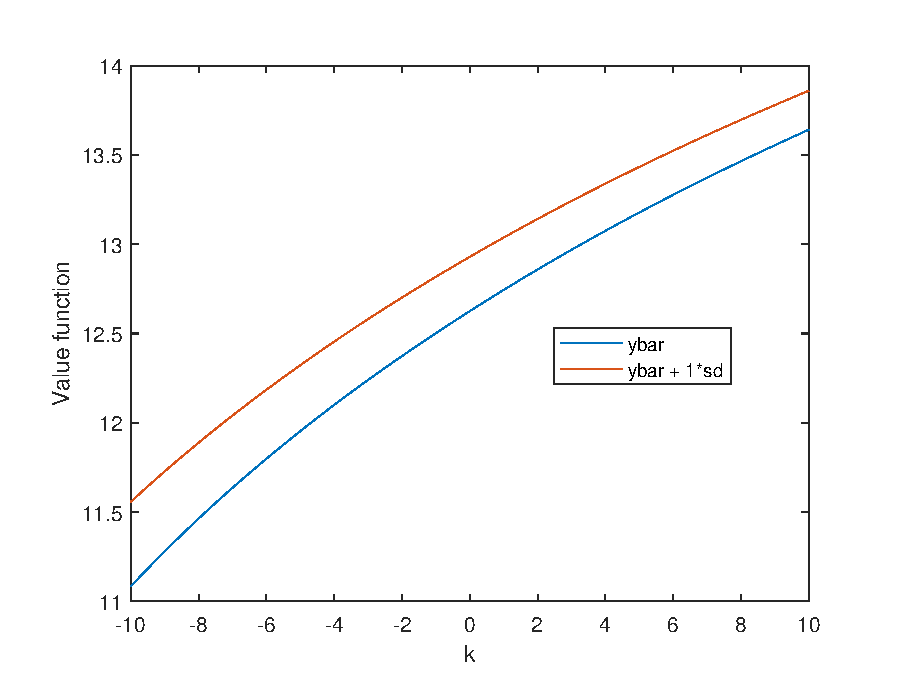
\includegraphics[height=2.5in]{value_function_51_gridpoints.eps}
	\caption{51 gridpoints}
		\label{fig:51gridpoints}
\end{figure*}

\begin{figure*}[t!]
	\centering
	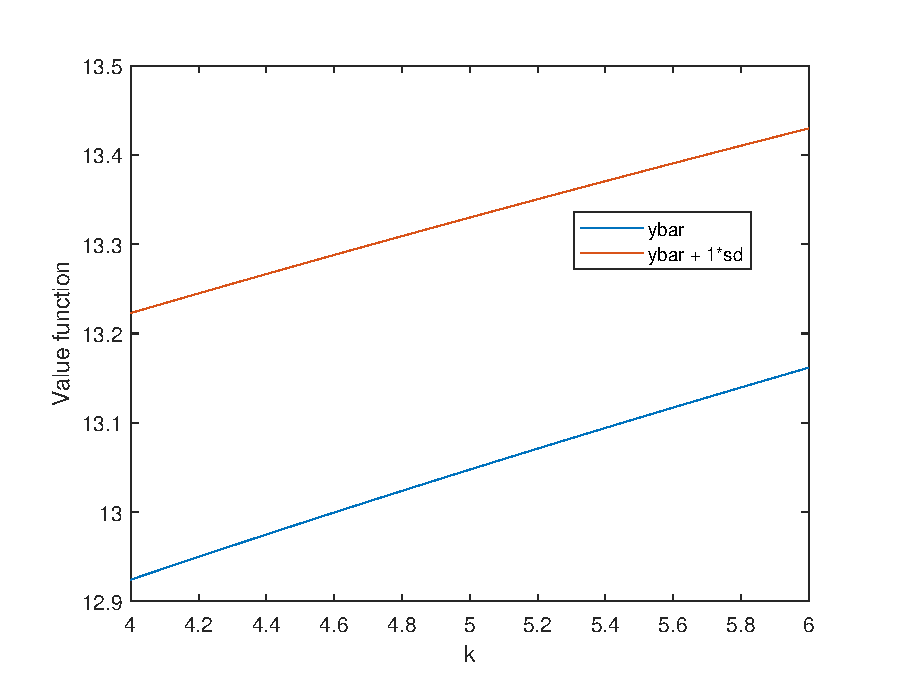
\includegraphics[height=2.5in]{value_function_101_gridpoints.eps}
	\caption{101 gridpoints}
	\label{fig:101gridpoints}
\end{figure*}

We can then use our value function to solve for optimal consumption and saving as a function of $k$. We compute this for 50 and 101 gridpoints for $k$ as shown in figures (\ref{fig:kp51gridpoints}) and (\ref{fig:kp101gridpoints}). We see that these plots are kinked, but are becoming smoother as we increase the number of grid points for k. If we increase the number of grid points to a large enough number, these will smooth out. \\



\begin{figure*}[t!]
	\centering
	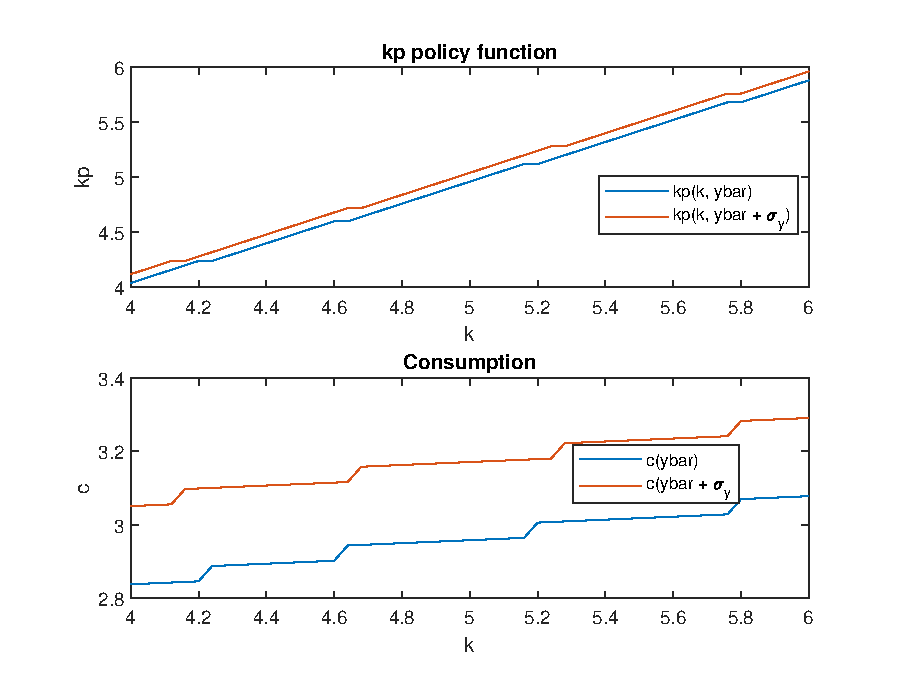
\includegraphics[height=2.5in]{k_and_p_51_gridpoints.eps}
	\caption{51 gridpoints}
	\label{fig:kp51gridpoints}
\end{figure*}

\begin{figure*}[t!]
	\centering
	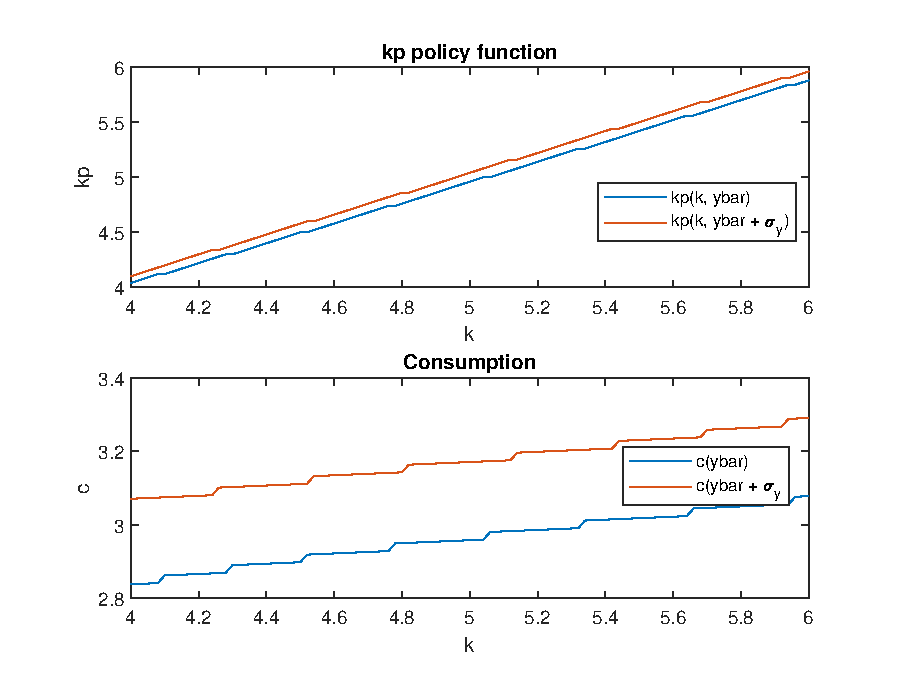
\includegraphics[height=2.5in]{k_and_p_101_gridpoints.eps}
	\caption{101 gridpoints}
	\label{fig:kp101gridpoints}
\end{figure*}

With our optimal consumption and savings decision rules we can simulate this economy using the AR(1) process specified above. We simulate the economy for 51 grid points for 5500 and 10500 periods (dropping the first 500 observations) then do the same for 101 grid points.  The table labeled Economy Simulation Summary Statistic compares the time series average, standard deviation, and persistance of consumption growth across the simulations. 
\begin{table}[!htbp] \centering 

	\begin{tabular}{@{\extracolsep{5pt}} c|ccc} 
		\\[-1.8ex]\hline 
		\hline \\[-1.8ex] 
		& Mean & Std. Deviation & Persistence\\ 
		\hline \\[-1.8ex] 
		51 grid points, 5000 simulations  & $0.000$ & $0.0781$ & $-0.0528$  \\ 
		51 grid points, 10000 simulations & $0.000$ & $0.0771$ & $-0.0113$ \\ 
		101 grid points, 5000 simulations & $-0.001$ & $0.0777$ & $-0.0264$ \\ 
		101 grid points, 10000 simulations & $0.000$ & $0.0775$ & $-0.0219$ \\ 
		\hline \\[-1.8ex] 
	\end{tabular} 
	\caption{Economy Simulation Summary Statistics} 
\end{table}

\end{document}


